\documentclass[11pt]{article}\usepackage[]{graphicx}\usepackage[]{color}
%% maxwidth is the original width if it is less than linewidth
%% otherwise use linewidth (to make sure the graphics do not exceed the margin)
\makeatletter
\def\maxwidth{ %
  \ifdim\Gin@nat@width>\linewidth
    \linewidth
  \else
    \Gin@nat@width
  \fi
}
\makeatother

\definecolor{fgcolor}{rgb}{0.345, 0.345, 0.345}
\newcommand{\hlnum}[1]{\textcolor[rgb]{0.686,0.059,0.569}{#1}}%
\newcommand{\hlstr}[1]{\textcolor[rgb]{0.192,0.494,0.8}{#1}}%
\newcommand{\hlcom}[1]{\textcolor[rgb]{0.678,0.584,0.686}{\textit{#1}}}%
\newcommand{\hlopt}[1]{\textcolor[rgb]{0,0,0}{#1}}%
\newcommand{\hlstd}[1]{\textcolor[rgb]{0.345,0.345,0.345}{#1}}%
\newcommand{\hlkwa}[1]{\textcolor[rgb]{0.161,0.373,0.58}{\textbf{#1}}}%
\newcommand{\hlkwb}[1]{\textcolor[rgb]{0.69,0.353,0.396}{#1}}%
\newcommand{\hlkwc}[1]{\textcolor[rgb]{0.333,0.667,0.333}{#1}}%
\newcommand{\hlkwd}[1]{\textcolor[rgb]{0.737,0.353,0.396}{\textbf{#1}}}%

\usepackage{framed}
\makeatletter
\newenvironment{kframe}{%
 \def\at@end@of@kframe{}%
 \ifinner\ifhmode%
  \def\at@end@of@kframe{\end{minipage}}%
  \begin{minipage}{\columnwidth}%
 \fi\fi%
 \def\FrameCommand##1{\hskip\@totalleftmargin \hskip-\fboxsep
 \colorbox{shadecolor}{##1}\hskip-\fboxsep
     % There is no \\@totalrightmargin, so:
     \hskip-\linewidth \hskip-\@totalleftmargin \hskip\columnwidth}%
 \MakeFramed {\advance\hsize-\width
   \@totalleftmargin\z@ \linewidth\hsize
   \@setminipage}}%
 {\par\unskip\endMakeFramed%
 \at@end@of@kframe}
\makeatother

\definecolor{shadecolor}{rgb}{.97, .97, .97}
\definecolor{messagecolor}{rgb}{0, 0, 0}
\definecolor{warningcolor}{rgb}{1, 0, 1}
\definecolor{errorcolor}{rgb}{1, 0, 0}
\newenvironment{knitrout}{}{} % an empty environment to be redefined in TeX

\usepackage{alltt}
\usepackage{amsmath}
\usepackage{stmaryrd}
\usepackage{bbm}
\usepackage{amsmath}
%\usepackage{mathtools}
\newcount\colveccount
\newcommand*\colvec[1]{
        \global\colveccount#1
        \begin{pmatrix}
        \colvecnext
}
\def\colvecnext#1{
        #1
        \global\advance\colveccount-1
        \ifnum\colveccount>0
                \\
                \expandafter\colvecnext
        \else
                \end{pmatrix}
        \fi
}
\newcommand{\argmin}{\arg\!\min}

\author{Thibault Doutre, Student ID 26980469}
\title{Problem Set 8\\ STAT243: Statistical Computing\\
University of California, Berkeley}
\date{\textit{December, 2015}}
\IfFileExists{upquote.sty}{\usepackage{upquote}}{}
\begin{document}
\maketitle

%%%%%%%%%%%%%%%%%%%%%%%%%%%%%%%%%%
\section{Bootstrap regression}
%%%%%%%%%%%%%%%%%%%%%%%%%%%%%%%%%%
We wish to compare the OLS estimator with one more robust method. Given $X$ and $Y$ such that $Y=X\beta+\epsilon$ with $\epsilon \sim N(0,1)$, the OLS estimator is obtained by minimizing the square loss and the robust method used here minimizes the absolute loss.\\
When treating the estimate $\beta$ as random variables, the Bootstrap can be used to estimate the confidence intervals.\\

\noindent
Let $B$ be the number of the bootstrapped samples. Let $X \in M_{n,p}(R)$ be the data and $Y \in R^n$ be the observations. The bootstrapped estimation of the regression parameter $\beta$ consists of the following:\\

For $b \in \{0..B-1\}$ do:
\begin{itemize}
\item Create $X_b \in M_{n,p}(R)$ and $Y_b \in R^{n}$ such that the lines of $X_b$ are sampled with replacement from the lines of $X$.
\item Estimate $\hat{\beta}_b$ with the regression method used.
\end{itemize}

\noindent
The bootstrapped mean estimator of $\beta$, say $\beta^*$ is the mean of the $\hat{\beta}_b$ for the OLS regression and the median of $\hat{\beta}_b$ for the robust regression. In order to have the confidence interval of the parameter of interest, one needs to compute the standard deviation of the parameters $\hat{\beta}_b$ now treated as random variables, say $SE \in R^p$. Then the confidence interval is then given by:
\begin{equation}
\left[\beta^*-SE*q_{1-\alpha/2}^{N(0,1)},\beta^*+SE*q_{1-\alpha/2}^{N(0,1)}\right]
\end{equation}

I chose to use robust LM from lmrob function in R. First, generate data and add some outliers.

\begin{knitrout}
\definecolor{shadecolor}{rgb}{0.969, 0.969, 0.969}\color{fgcolor}\begin{kframe}
\begin{alltt}
\hlkwd{set.seed}\hlstd{(}\hlnum{1}\hlstd{)}
\hlkwd{library}\hlstd{(robust)}
\end{alltt}


{\ttfamily\noindent\itshape\color{messagecolor}{\#\# Loading required package: fit.models\\\#\# Loading required package: lattice\\\#\# Loading required package: MASS\\\#\# Loading required package: robustbase\\\#\# Loading required package: rrcov\\\#\# Scalable Robust Estimators with High Breakdown Point (version 1.3-8)}}\begin{alltt}
\hlkwd{options}\hlstd{(}\hlkwc{warn}\hlstd{=}\hlopt{-}\hlnum{1}\hlstd{)}

\hlcom{# Generate data }
\hlstd{n}\hlkwb{=}\hlnum{30}
\hlstd{p}\hlkwb{=}\hlnum{4}
\hlstd{beta} \hlkwb{=} \hlkwd{matrix}\hlstd{(}\hlkwd{c}\hlstd{(}\hlnum{.5}\hlstd{,}\hlnum{1}\hlstd{,}\hlnum{0}\hlstd{,}\hlnum{0}\hlstd{),}\hlkwc{ncol}\hlstd{=}\hlnum{1}\hlstd{)}
\hlstd{X} \hlkwb{=} \hlkwd{cbind}\hlstd{(}\hlnum{1}\hlstd{,}\hlkwd{rnorm}\hlstd{(n,}\hlkwc{sd}\hlstd{=}\hlnum{4}\hlstd{),}\hlkwd{rnorm}\hlstd{(n,}\hlkwc{sd}\hlstd{=}\hlnum{.2}\hlstd{),}\hlkwd{rnorm}\hlstd{(n,}\hlkwc{sd}\hlstd{=}\hlnum{.2}\hlstd{))}
\hlstd{Y} \hlkwb{=} \hlstd{X}\hlopt\hlstd{beta}\hlopt{+}\hlkwd{matrix}\hlstd{(}\hlkwd{rnorm}\hlstd{(n),}\hlkwc{ncol}\hlstd{=}\hlnum{1}\hlstd{)} \hlcom{#Good data}
\hlstd{Y[}\hlkwd{sample}\hlstd{(}\hlnum{1}\hlopt{:}\hlstd{n,n}\hlopt{/}\hlnum{10}\hlstd{)]} \hlkwb{=} \hlstd{Y[}\hlkwd{sample}\hlstd{(}\hlnum{1}\hlopt{:}\hlstd{n,n}\hlopt{/}\hlnum{10}\hlstd{)]} \hlopt{+}
  \hlkwd{rnorm}\hlstd{(}\hlnum{0}\hlstd{,}\hlnum{40}\hlstd{,}\hlkwc{n}\hlstd{=n}\hlopt{/}\hlnum{10}\hlstd{)} \hlcom{#Bad data 10%}
\hlkwd{plot}\hlstd{(X[,}\hlnum{2}\hlstd{],Y,}\hlkwc{main}\hlstd{=}\hlstr{"Generated data"}\hlstd{)}
\end{alltt}
\end{kframe}
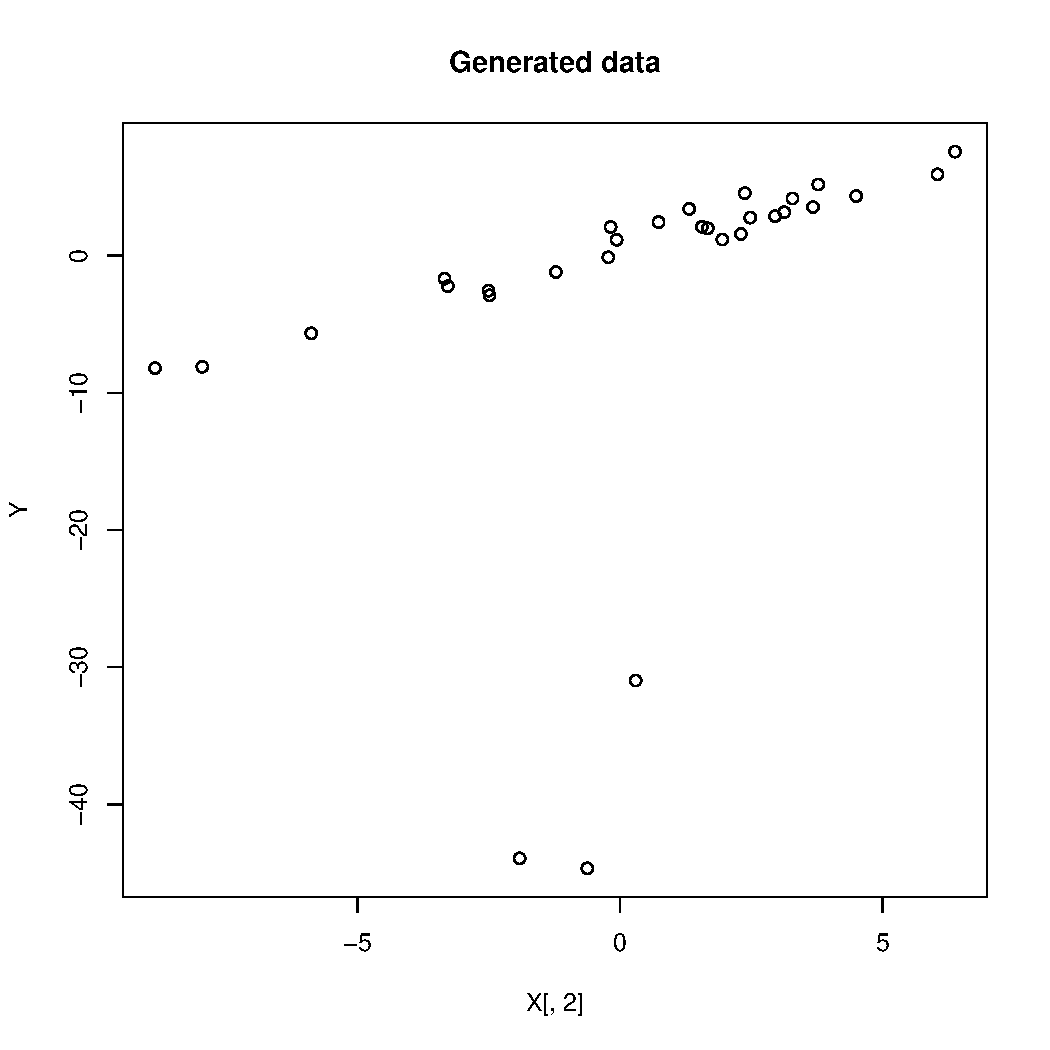
\includegraphics[width=\maxwidth]{figure/unnamed-chunk-1-1} 

\end{knitrout}

Then, I compute the OLS estimation, choosing $B=1000$.
\begin{knitrout}
\definecolor{shadecolor}{rgb}{0.969, 0.969, 0.969}\color{fgcolor}\begin{kframe}
\begin{alltt}
\hlcom{################# OLS ######################}
\hlkwd{plot}\hlstd{(X[,}\hlnum{2}\hlstd{],Y,}\hlkwc{main}\hlstd{=}\hlstr{"OLS Regression"}\hlstd{)}

\hlcom{# Bootsrap sample}
\hlstd{B}\hlkwb{=}\hlnum{1000}
\hlstd{r}\hlkwb{=}\hlstd{n}
\hlstd{OLSbetastar}\hlkwb{=}\hlkwd{matrix}\hlstd{(}\hlkwc{nrow}\hlstd{=B,}\hlkwc{ncol}\hlstd{=p)}
\hlkwa{for} \hlstd{(b} \hlkwa{in} \hlnum{1}\hlopt{:}\hlstd{B)\{}
  \hlstd{s}\hlkwb{=}\hlkwd{sample}\hlstd{(}\hlnum{1}\hlopt{:}\hlstd{n,r,}\hlkwc{replace}\hlstd{=T)}
  \hlstd{Xstar}\hlkwb{=}\hlstd{X[s,]}
  \hlstd{Ystar}\hlkwb{=}\hlstd{Y[s]}
  \hlstd{OLSbetastar[b,]}\hlkwb{=}\hlkwd{lm}\hlstd{(Ystar}\hlopt{~}\hlstd{Xstar[,}\hlopt{-}\hlnum{1}\hlstd{])}\hlopt{$}\hlstd{coefficients}
\hlstd{\}}

\hlcom{# Bootsrapped estimates}
\hlstd{OLSbetastar_hat}\hlkwb{=}\hlkwd{apply}\hlstd{(OLSbetastar,}\hlnum{2}\hlstd{,mean)}
\hlkwd{sum}\hlstd{(}\hlkwd{abs}\hlstd{(Y}\hlopt{-}\hlstd{X}\hlopt\hlstd{OLSbetastar_hat))} \hlcom{# Absolute error}
\end{alltt}
\begin{verbatim}
## [1] 214.9669
\end{verbatim}
\begin{alltt}
\hlkwa{for} \hlstd{(row} \hlkwa{in} \hlnum{1}\hlopt{:}\hlstd{n)\{}
  \hlkwd{abline}\hlstd{(OLSbetastar[row,}\hlnum{1}\hlopt{:}\hlnum{2}\hlstd{],}\hlkwc{col}\hlstd{=}\hlstr{"darkgray"}\hlstd{,}\hlkwc{lwd}\hlstd{=}\hlnum{0.3}\hlstd{)}
\hlstd{\}}
\hlkwd{abline}\hlstd{(OLSbetastar_hat[}\hlnum{1}\hlopt{:}\hlnum{2}\hlstd{],}\hlkwc{lwd}\hlstd{=}\hlnum{1.3}\hlstd{)}

\hlcom{# Bootstrapped confint 95%}
\hlstd{SE}\hlkwb{=}\hlkwd{apply}\hlstd{(OLSbetastar,}\hlnum{2}\hlstd{,sd)}
\hlstd{borne_sup}\hlkwb{=}\hlstd{OLSbetastar_hat}\hlopt{+}\hlkwd{qnorm}\hlstd{(}\hlnum{1}\hlopt{-}\hlnum{.05}\hlopt{/}\hlnum{2}\hlstd{)}\hlopt{*}\hlstd{SE}
\hlstd{borne_inf}\hlkwb{=}\hlstd{OLSbetastar_hat}\hlopt{-}\hlkwd{qnorm}\hlstd{(}\hlnum{1}\hlopt{-}\hlnum{.05}\hlopt{/}\hlnum{2}\hlstd{)}\hlopt{*}\hlstd{SE}
\hlkwd{abline}\hlstd{(borne_sup[}\hlnum{1}\hlopt{:}\hlnum{2}\hlstd{],}\hlkwc{lty}\hlstd{=}\hlnum{3}\hlstd{)}
\hlkwd{abline}\hlstd{(borne_inf[}\hlnum{1}\hlopt{:}\hlnum{2}\hlstd{],}\hlkwc{lty}\hlstd{=}\hlnum{3}\hlstd{)}

\hlcom{# True beta}
\hlkwd{abline}\hlstd{(beta[}\hlnum{1}\hlopt{:}\hlnum{2}\hlstd{],}\hlkwc{col}\hlstd{=}\hlstr{"blue"}\hlstd{)}

\hlkwd{legend}\hlstd{(}\hlstr{"bottomleft"}\hlstd{,}\hlkwd{c}\hlstd{(}\hlstr{"Truth"}\hlstd{,}\hlstr{"Estimate"}\hlstd{,}\hlstr{"confidence interval"}\hlstd{),}
       \hlkwc{lty}\hlstd{=}\hlkwd{c}\hlstd{(}\hlnum{1}\hlstd{,}\hlnum{1}\hlstd{,}\hlnum{3}\hlstd{),}\hlkwc{col}\hlstd{=}\hlkwd{c}\hlstd{(}\hlstr{"blue"}\hlstd{,}\hlstr{"black"}\hlstd{,}\hlstr{"black"}\hlstd{))}
\end{alltt}
\end{kframe}
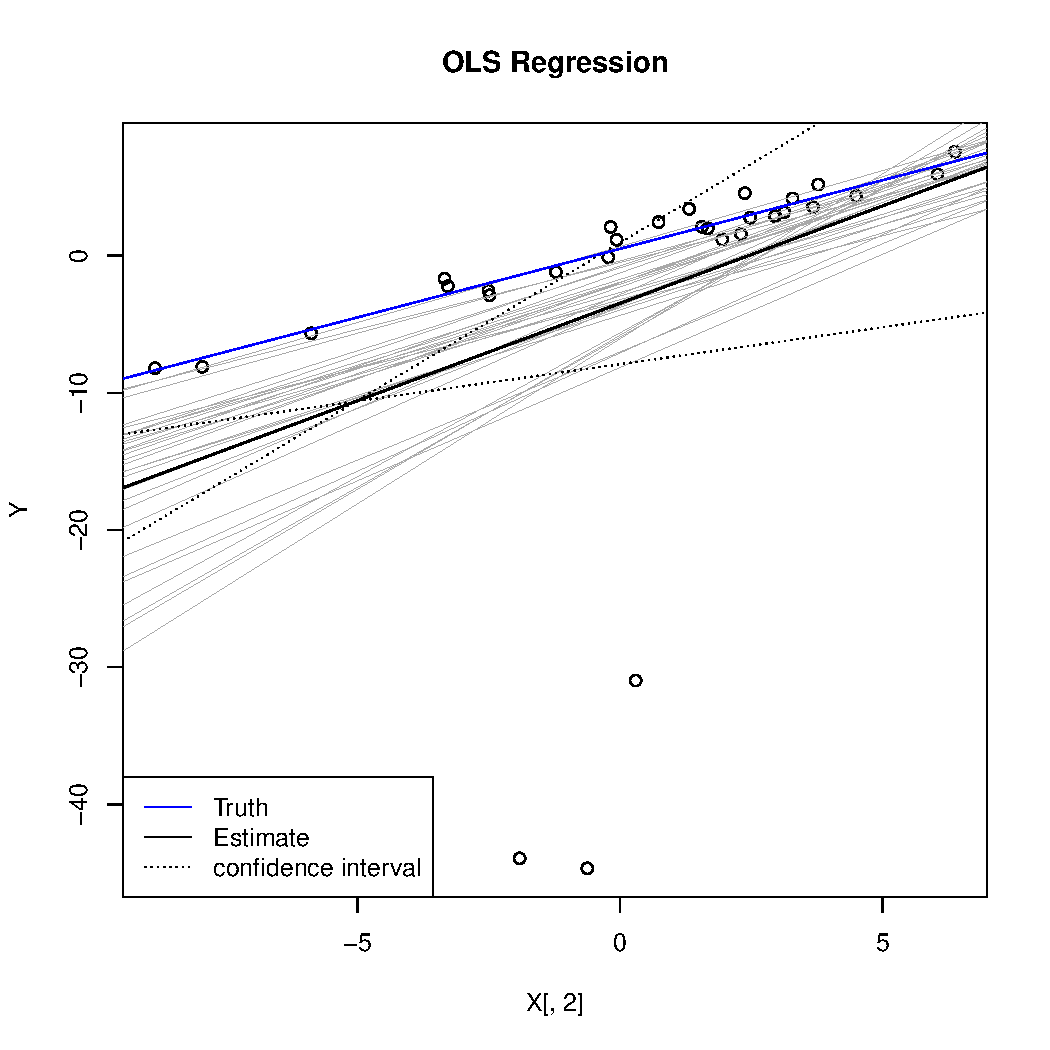
\includegraphics[width=\maxwidth]{figure/unnamed-chunk-2-1} 
\begin{kframe}\begin{alltt}
\hlcom{# Coverage prediction}
\hlkwd{mean}\hlstd{(}\hlkwd{apply}\hlstd{(OLSbetastar,}\hlnum{1}\hlstd{,}\hlkwa{function}\hlstd{(}\hlkwc{row}\hlstd{)} \hlkwd{Reduce}\hlstd{(}\hlstr{'*'}\hlstd{,row}\hlopt{>}\hlstd{borne_inf} \hlopt{&&} \hlstd{row}\hlopt{<}\hlstd{borne_sup)))}
\end{alltt}
\begin{verbatim}
## [1] 0.962
\end{verbatim}
\end{kframe}
\end{knitrout}
We can see that the confidence interval is indeed 0.95.
To compare the robust method with standard OLS, I do the exact same steps than before with the robust method.

\begin{knitrout}
\definecolor{shadecolor}{rgb}{0.969, 0.969, 0.969}\color{fgcolor}\begin{kframe}
\begin{alltt}
\hlcom{################# ROBUST ######################}
\hlkwd{plot}\hlstd{(X[,}\hlnum{2}\hlstd{],Y,}\hlkwc{main}\hlstd{=}\hlstr{"Robust Regression"}\hlstd{)}

\hlcom{# Bootsrap sample}
\hlstd{B}\hlkwb{=}\hlnum{1000}
\hlstd{r}\hlkwb{=}\hlstd{n}
\hlstd{betastar}\hlkwb{=}\hlkwd{matrix}\hlstd{(}\hlkwc{nrow}\hlstd{=B,}\hlkwc{ncol}\hlstd{=p)}
\hlkwa{for} \hlstd{(b} \hlkwa{in} \hlnum{1}\hlopt{:}\hlstd{B)\{}
  \hlstd{s}\hlkwb{=}\hlkwd{sample}\hlstd{(}\hlnum{1}\hlopt{:}\hlstd{n,r,}\hlkwc{replace}\hlstd{=T)}
  \hlstd{Xstar}\hlkwb{=}\hlstd{X[s,]}
  \hlstd{Ystar}\hlkwb{=}\hlstd{Y[s]}
  \hlstd{betastar[b,]}\hlkwb{=}\hlkwd{lmrob}\hlstd{(Ystar}\hlopt{~}\hlstd{Xstar[,}\hlopt{-}\hlnum{1}\hlstd{],}\hlkwc{tau}\hlstd{=}\hlnum{.5}\hlstd{)}\hlopt{$}\hlstd{coefficients}
\hlstd{\}}

\hlcom{# Bootsrapped estimates}
\hlstd{betastar_hat}\hlkwb{=}\hlkwd{apply}\hlstd{(betastar,}\hlnum{2}\hlstd{,mean)}
\hlkwd{sum}\hlstd{(}\hlkwd{abs}\hlstd{(Y}\hlopt{-}\hlstd{X}\hlopt\hlstd{betastar_hat))} \hlcom{# Absolute error}
\end{alltt}
\begin{verbatim}
## [1] 139.0308
\end{verbatim}
\begin{alltt}
\hlkwa{for} \hlstd{(row} \hlkwa{in} \hlnum{1}\hlopt{:}\hlstd{n)\{}
  \hlkwd{abline}\hlstd{(betastar[row,}\hlnum{1}\hlopt{:}\hlnum{2}\hlstd{],}\hlkwc{col}\hlstd{=}\hlstr{"darkgray"}\hlstd{,}\hlkwc{lwd}\hlstd{=}\hlnum{0.3}\hlstd{)}
\hlstd{\}}
\hlkwd{abline}\hlstd{(betastar_hat[}\hlnum{1}\hlopt{:}\hlnum{2}\hlstd{],}\hlkwc{lwd}\hlstd{=}\hlnum{1.3}\hlstd{)}

\hlcom{# Bootstrapped confint 95%}
\hlstd{SE}\hlkwb{=}\hlkwd{apply}\hlstd{(betastar,}\hlnum{2}\hlstd{,sd)}
\hlstd{borne_sup}\hlkwb{=}\hlstd{betastar_hat}\hlopt{+}\hlkwd{qnorm}\hlstd{(}\hlnum{1}\hlopt{-}\hlnum{.05}\hlopt{/}\hlnum{2}\hlstd{)}\hlopt{*}\hlstd{SE}
\hlstd{borne_inf}\hlkwb{=}\hlstd{betastar_hat}\hlopt{-}\hlkwd{qnorm}\hlstd{(}\hlnum{1}\hlopt{-}\hlnum{.05}\hlopt{/}\hlnum{2}\hlstd{)}\hlopt{*}\hlstd{SE}
\hlkwd{abline}\hlstd{(borne_sup[}\hlnum{1}\hlopt{:}\hlnum{2}\hlstd{],}\hlkwc{lty}\hlstd{=}\hlnum{3}\hlstd{)}
\hlkwd{abline}\hlstd{(borne_inf[}\hlnum{1}\hlopt{:}\hlnum{2}\hlstd{],}\hlkwc{lty}\hlstd{=}\hlnum{3}\hlstd{)}

\hlcom{# True beta}
\hlkwd{abline}\hlstd{(beta[}\hlnum{1}\hlopt{:}\hlnum{2}\hlstd{],}\hlkwc{col}\hlstd{=}\hlstr{"blue"}\hlstd{)}

\hlkwd{legend}\hlstd{(}\hlstr{"bottomleft"}\hlstd{,}\hlkwd{c}\hlstd{(}\hlstr{"Truth"}\hlstd{,}\hlstr{"Estimate"}\hlstd{,}\hlstr{"confidence interval"}\hlstd{),}
       \hlkwc{lty}\hlstd{=}\hlkwd{c}\hlstd{(}\hlnum{1}\hlstd{,}\hlnum{1}\hlstd{,}\hlnum{3}\hlstd{),}\hlkwc{col}\hlstd{=}\hlkwd{c}\hlstd{(}\hlstr{"blue"}\hlstd{,}\hlstr{"black"}\hlstd{,}\hlstr{"black"}\hlstd{))}
\end{alltt}
\end{kframe}
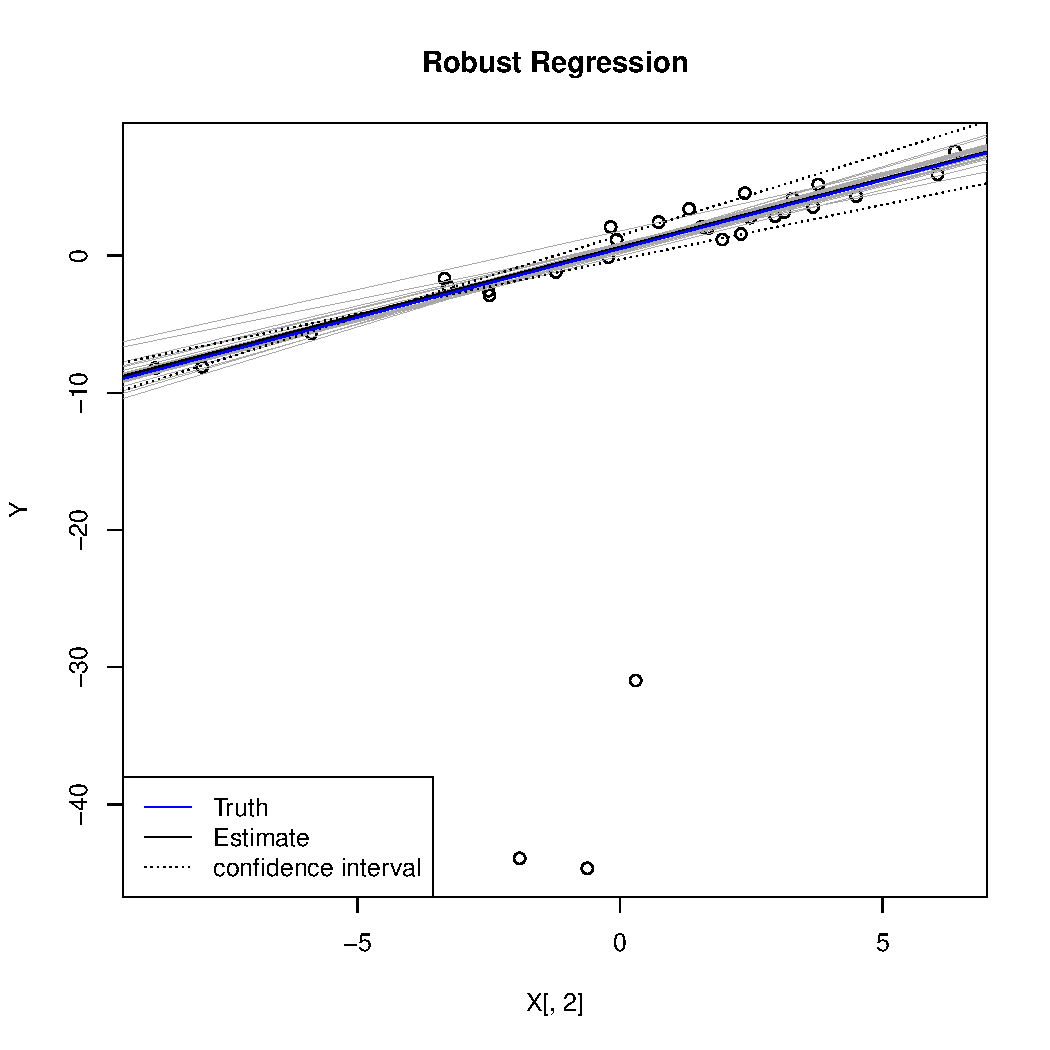
\includegraphics[width=\maxwidth]{figure/unnamed-chunk-3-1} 
\begin{kframe}\begin{alltt}
\hlcom{# Coverage prediction}
\hlkwd{mean}\hlstd{(}\hlkwd{apply}\hlstd{(betastar,}\hlnum{1}\hlstd{,}\hlkwa{function}\hlstd{(}\hlkwc{row}\hlstd{)} \hlkwd{Reduce}\hlstd{(}\hlstr{'*'}\hlstd{,row}\hlopt{>}\hlstd{borne_inf} \hlopt{&&} \hlstd{row}\hlopt{<}\hlstd{borne_sup)))}
\end{alltt}
\begin{verbatim}
## [1] 0.985
\end{verbatim}
\end{kframe}
\end{knitrout}

And I finally report the absolute errors:
\begin{knitrout}
\definecolor{shadecolor}{rgb}{0.969, 0.969, 0.969}\color{fgcolor}\begin{kframe}
\begin{alltt}
\hlkwd{sum}\hlstd{(}\hlkwd{abs}\hlstd{(Y}\hlopt{-}\hlstd{X}\hlopt\hlstd{betastar_hat))} \hlcom{# LMROB_boot Absolute error}
\end{alltt}
\begin{verbatim}
## [1] 139.0308
\end{verbatim}
\begin{alltt}
\hlkwd{sum}\hlstd{(}\hlkwd{abs}\hlstd{(Y}\hlopt{-}\hlstd{X}\hlopt\hlstd{OLSbetastar_hat))} \hlcom{# OLS Absolute error}
\end{alltt}
\begin{verbatim}
## [1] 214.9669
\end{verbatim}
\end{kframe}
\end{knitrout}
We note that theOLS estimate is worse than the robust one because of these these outliers.\\

%%%%%%%%%%%%%%%%%%%%%%%%%%%%%%%%%%
\section{Monte Carlo}
%%%%%%%%%%%%%%%%%%%%%%%%%%%%%%%%%%
The tail of the Pareto decay more slowly than that of an exponential distribution. Indeed, when taking the ratio of the tails of the distributions, we have:
\begin{equation}
\frac{e^{-\lambda x}}{\alpha^{\beta}/x^{\beta}}=\frac{x^{\beta} e^{-\lambda x}}{ \alpha^{\beta}} \xrightarrow[x \to \infty]{}0
\end{equation}
We can confirm this mathematical statement when plotting the curves:
\begin{knitrout}
\definecolor{shadecolor}{rgb}{0.969, 0.969, 0.969}\color{fgcolor}\begin{kframe}
\begin{alltt}
\hlkwd{library}\hlstd{(actuar)}
\end{alltt}


{\ttfamily\noindent\itshape\color{messagecolor}{\#\# \\\#\# Attaching package: 'actuar'\\\#\# \\\#\# The following object is masked from 'package:grDevices':\\\#\# \\\#\#\ \ \ \  cm}}\end{kframe}
\end{knitrout}
\begin{knitrout}
\definecolor{shadecolor}{rgb}{0.969, 0.969, 0.969}\color{fgcolor}\begin{kframe}
\begin{alltt}
\hlcom{# Plot}
\hlstd{x}\hlkwb{=}\hlkwd{seq}\hlstd{(}\hlnum{1}\hlstd{,}\hlnum{10}\hlstd{,}\hlkwc{by}\hlstd{=}\hlnum{0.1}\hlstd{)}
\hlkwd{plot}\hlstd{(x,}\hlkwd{dpareto}\hlstd{(x,}\hlkwc{shape}\hlstd{=}\hlnum{3}\hlstd{,}\hlkwc{scale}\hlstd{=}\hlnum{2}\hlstd{),}\hlkwc{type}\hlstd{=}\hlstr{"l"}\hlstd{,}\hlkwc{col}\hlstd{=}\hlstr{"red"}\hlstd{,}\hlkwc{ylab}\hlstd{=}
       \hlstr{"density"}\hlstd{,}\hlkwc{main}\hlstd{=}\hlstr{"Density comparison"}\hlstd{)}
\hlkwd{lines}\hlstd{(x,}\hlkwd{dexp}\hlstd{(x),}\hlkwc{col}\hlstd{=}\hlstr{"blue"}\hlstd{)}
\hlkwd{legend}\hlstd{(}\hlstr{"topright"}\hlstd{,}\hlkwd{c}\hlstd{(}\hlstr{"pareto(2,3)"}\hlstd{,}\hlstr{"exp(1)"}\hlstd{),}\hlkwc{col}\hlstd{=}\hlkwd{c}\hlstd{(}\hlstr{"red"}\hlstd{,}\hlstr{"blue"}\hlstd{)}
       \hlstd{,}\hlkwc{pch}\hlstd{=}\hlstr{"--"}\hlstd{)}
\end{alltt}
\end{kframe}
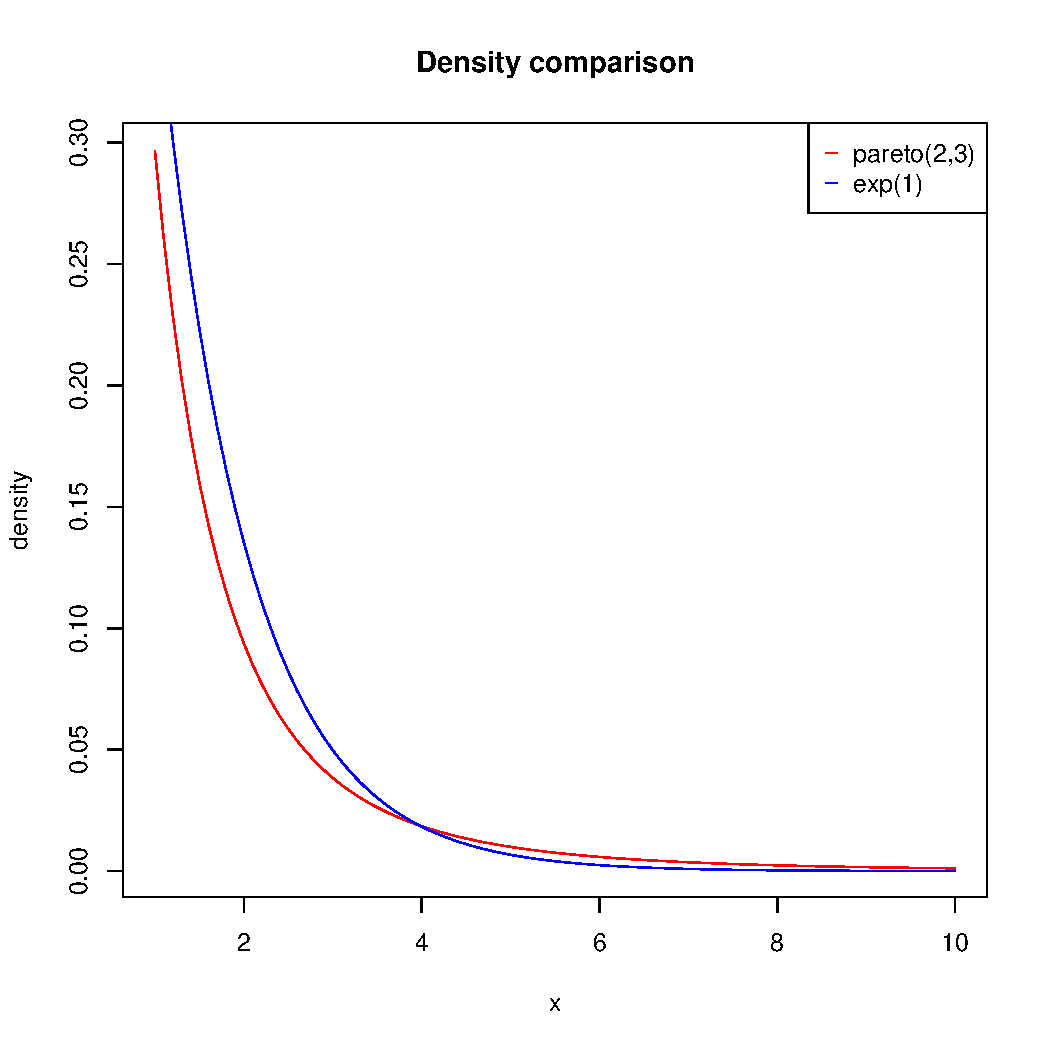
\includegraphics[width=\maxwidth]{figure/unnamed-chunk-6-1} 

\end{knitrout}

\subsection{Sampling density with heavier tail}
If we sample the shifted exponential distribution with the Pareto distribution, we have:
\begin{knitrout}
\definecolor{shadecolor}{rgb}{0.969, 0.969, 0.969}\color{fgcolor}\begin{kframe}
\begin{alltt}
\hlcom{# Moment estimation}
\hlstd{f} \hlkwb{=} \hlkwa{function}\hlstd{(}\hlkwc{x}\hlstd{)\{}
  \hlkwd{dexp}\hlstd{(x}\hlopt{-}\hlnum{2}\hlstd{)}
\hlstd{\}}
\hlstd{g} \hlkwb{=} \hlkwa{function}\hlstd{(}\hlkwc{x}\hlstd{)\{}
  \hlkwd{dpareto}\hlstd{(x,}\hlkwc{shape}\hlstd{=}\hlnum{3}\hlstd{,}\hlkwc{scale}\hlstd{=}\hlnum{2}\hlstd{)}
\hlstd{\}}
\hlstd{w}\hlkwb{=}\hlkwa{function}\hlstd{(}\hlkwc{x}\hlstd{)\{}
  \hlkwd{f}\hlstd{(x)}\hlopt{/}\hlkwd{g}\hlstd{(x)}
\hlstd{\}}
\hlstd{h1}\hlkwb{=}\hlkwa{function}\hlstd{(}\hlkwc{x}\hlstd{)\{}
  \hlstd{x}\hlopt{*}\hlkwd{w}\hlstd{(x)}
\hlstd{\}}
\hlstd{h2}\hlkwb{=}\hlkwa{function}\hlstd{(}\hlkwc{x}\hlstd{)\{}
  \hlstd{(x}\hlopt{^}\hlnum{2}\hlstd{)}\hlopt{*}\hlkwd{w}\hlstd{(x)}
\hlstd{\}}

\hlstd{m}\hlkwb{=}\hlnum{10000}
\hlstd{sample}\hlkwb{=}\hlkwd{rpareto}\hlstd{(m,}\hlkwc{shape}\hlstd{=}\hlnum{3}\hlstd{,}\hlkwc{scale}\hlstd{=}\hlnum{2}\hlstd{)}

\hlcom{#E(X)}
\hlkwd{mean}\hlstd{(}\hlkwd{h1}\hlstd{(sample))}
\end{alltt}
\begin{verbatim}
## [1] 2.933696
\end{verbatim}
\begin{alltt}
\hlcom{#E(X2)}
\hlkwd{mean}\hlstd{(}\hlkwd{h2}\hlstd{(sample))}
\end{alltt}
\begin{verbatim}
## [1] 9.89575
\end{verbatim}
\end{kframe}
\end{knitrout}

\begin{knitrout}
\definecolor{shadecolor}{rgb}{0.969, 0.969, 0.969}\color{fgcolor}\begin{kframe}
\begin{alltt}
\hlcom{#plot}
\hlkwd{plot.new}\hlstd{()}
\hlkwd{par}\hlstd{(}\hlkwc{mfrow}\hlstd{=}\hlkwd{c}\hlstd{(}\hlnum{1}\hlstd{,}\hlnum{3}\hlstd{))}
\hlkwd{hist}\hlstd{(}\hlkwd{h1}\hlstd{(sample),}\hlkwc{xlab}\hlstd{=}\hlstr{"xf(x)/g(x)"}\hlstd{,}\hlkwc{main}\hlstd{=}\hlstr{""}\hlstd{)}
\hlkwd{hist}\hlstd{(}\hlkwd{h2}\hlstd{(sample),}\hlkwc{xlab}\hlstd{=}\hlstr{"x2f(x)/g(x)"}\hlstd{,}\hlkwc{main}\hlstd{=}\hlstr{""}\hlstd{)}
\hlkwd{hist}\hlstd{(}\hlkwd{w}\hlstd{(sample),}\hlkwc{xlab}\hlstd{=}\hlstr{"f(x)/g(x)"}\hlstd{,}\hlkwc{main}\hlstd{=}\hlstr{""}\hlstd{)}
\hlkwd{title}\hlstd{(}\hlstr{"Monte Carlo Histograms"}\hlstd{,}\hlkwc{outer}\hlstd{=T,}\hlkwc{line}\hlstd{=}\hlopt{-}\hlnum{3}\hlstd{)}
\end{alltt}
\end{kframe}
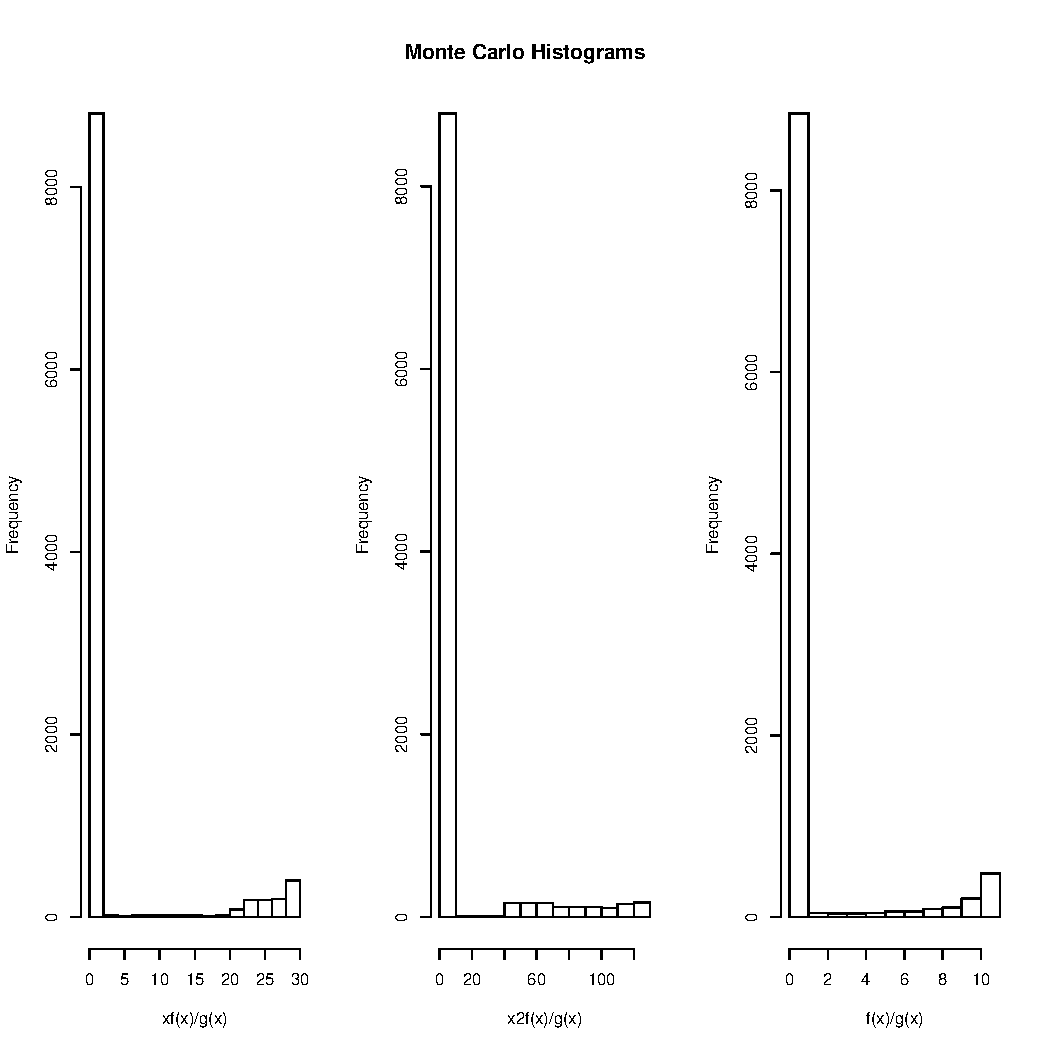
\includegraphics[width=\maxwidth]{figure/unnamed-chunk-8-1} 

\end{knitrout}

We can see that there is not any extreme weights values, according to the range of the histogram or by computing the maximum of the weights:
\begin{knitrout}
\definecolor{shadecolor}{rgb}{0.969, 0.969, 0.969}\color{fgcolor}\begin{kframe}
\begin{alltt}
\hlcom{#maxweight}
\hlkwd{max}\hlstd{(}\hlkwd{w}\hlstd{(sample))}
\end{alltt}
\begin{verbatim}
## [1] 10.66666
\end{verbatim}
\end{kframe}
\end{knitrout}
\subsection{Sampling density with lighter tail}
Here, we can see that we do have extreme weights in some cases. When sampling with the shifted exponential distribution with the Pareto, we have:
\begin{knitrout}
\definecolor{shadecolor}{rgb}{0.969, 0.969, 0.969}\color{fgcolor}\begin{kframe}
\begin{alltt}
\hlcom{# Exchange f and g}
\hlstd{f} \hlkwb{=} \hlkwa{function}\hlstd{(}\hlkwc{x}\hlstd{)\{}
  \hlkwd{dpareto}\hlstd{(x,}\hlkwc{shape}\hlstd{=}\hlnum{3}\hlstd{,}\hlkwc{scale}\hlstd{=}\hlnum{2}\hlstd{)}
\hlstd{\}}
\hlstd{g} \hlkwb{=} \hlkwa{function}\hlstd{(}\hlkwc{x}\hlstd{)\{}
  \hlkwd{dexp}\hlstd{(x}\hlopt{-}\hlnum{2}\hlstd{)}
\hlstd{\}}
\hlstd{w}\hlkwb{=}\hlkwa{function}\hlstd{(}\hlkwc{x}\hlstd{)\{}
  \hlkwd{f}\hlstd{(x)}\hlopt{/}\hlkwd{g}\hlstd{(x)}
\hlstd{\}}
\hlstd{h1}\hlkwb{=}\hlkwa{function}\hlstd{(}\hlkwc{x}\hlstd{)\{}
  \hlstd{x}\hlopt{*}\hlkwd{w}\hlstd{(x)}
\hlstd{\}}
\hlstd{h2}\hlkwb{=}\hlkwa{function}\hlstd{(}\hlkwc{x}\hlstd{)\{}
  \hlstd{(x}\hlopt{^}\hlnum{2}\hlstd{)}\hlopt{*}\hlkwd{w}\hlstd{(x)}
\hlstd{\}}
\hlstd{m}\hlkwb{=}\hlnum{10000}
\hlkwd{set.seed}\hlstd{(}\hlnum{6}\hlstd{)}
\hlstd{sample}\hlkwb{=}\hlkwd{rexp}\hlstd{(m)}\hlopt{+}\hlnum{2}
\hlcom{#E(X)}
\hlkwd{mean}\hlstd{(}\hlkwd{h1}\hlstd{(sample))}
\end{alltt}
\begin{verbatim}
## [1] 1.142526
\end{verbatim}
\begin{alltt}
\hlcom{#E(X2)}
\hlkwd{mean}\hlstd{(}\hlkwd{h2}\hlstd{(sample))}
\end{alltt}
\begin{verbatim}
## [1] 13.76207
\end{verbatim}
\end{kframe}
\end{knitrout}

\begin{knitrout}
\definecolor{shadecolor}{rgb}{0.969, 0.969, 0.969}\color{fgcolor}\begin{kframe}
\begin{alltt}
\hlcom{#plot}
\hlkwd{plot.new}\hlstd{()}
\hlkwd{par}\hlstd{(}\hlkwc{mfrow}\hlstd{=}\hlkwd{c}\hlstd{(}\hlnum{1}\hlstd{,}\hlnum{3}\hlstd{))}
\hlkwd{hist}\hlstd{(}\hlkwd{h1}\hlstd{(sample),}\hlkwc{xlab}\hlstd{=}\hlstr{"xf(x)/g(x)"}\hlstd{,}\hlkwc{main}\hlstd{=}\hlstr{""}\hlstd{)}
\hlkwd{hist}\hlstd{(}\hlkwd{h2}\hlstd{(sample),}\hlkwc{xlab}\hlstd{=}\hlstr{"xf(x)/g(x)"}\hlstd{,}\hlkwc{main}\hlstd{=}\hlstr{""}\hlstd{)}
\hlkwd{hist}\hlstd{(} \hlkwd{w}\hlstd{(sample),}\hlkwc{xlab}\hlstd{=}\hlstr{"f(x)/g(x) "}\hlstd{,}\hlkwc{main}\hlstd{=}\hlstr{""}\hlstd{)}
\hlkwd{title}\hlstd{(}\hlstr{"Monte Carlo Histograms"}\hlstd{,}\hlkwc{outer}\hlstd{=T,}\hlkwc{line}\hlstd{=}\hlopt{-}\hlnum{3}\hlstd{)}
\end{alltt}
\end{kframe}
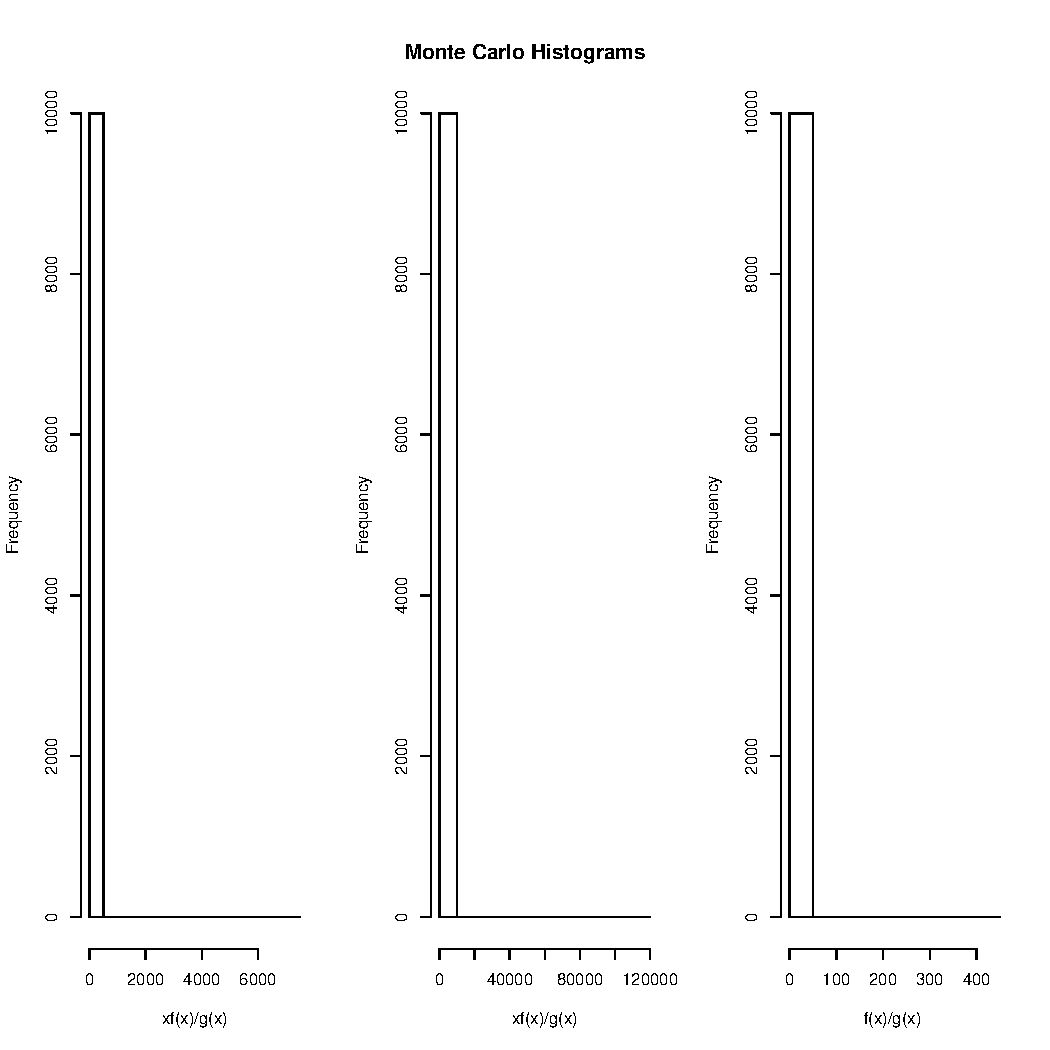
\includegraphics[width=\maxwidth]{figure/unnamed-chunk-11-1} 
\begin{kframe}\begin{alltt}
\hlkwd{par}\hlstd{(}\hlkwc{mfrow}\hlstd{=}\hlkwd{c}\hlstd{(}\hlnum{1}\hlstd{,}\hlnum{1}\hlstd{))}
\end{alltt}
\end{kframe}
\end{knitrout}

\begin{knitrout}
\definecolor{shadecolor}{rgb}{0.969, 0.969, 0.969}\color{fgcolor}\begin{kframe}
\begin{alltt}
\hlcom{#maxweight}
\hlkwd{max}\hlstd{(}\hlkwd{w}\hlstd{(sample))}
\end{alltt}
\begin{verbatim}
## [1] 434.0526
\end{verbatim}
\end{kframe}
\end{knitrout}
It is actually important to have the ratio of the density of interest over the sampling density upper bounded in absolute value.

%%%%%%%%%%%%%%%%%%%%%%%%%%%%%%%%%%
\section{EM}
%%%%%%%%%%%%%%%%%%%%%%%%%%%%%%%%%%
The probit regression can be rewritten as:
\begin{align}
Z_i&=X_i^T\beta+\epsilon \hspace{2cm} \epsilon  \sim N(0,1)
\nonumber\\%%%%%%%%%%%%%%%%%%%%%%%%%%%%%%%%%%%%%
Y_i&=I(Z_i>0)
\end{align}
\noindent
The expected complete log-likelihood is:
\begin{align}
Q(\beta)&=-\frac{1}{2}E[ (Z-X\beta)^T(Z-X\beta)|Y,\beta] + cst
\end{align}
Assuming that we can interchange the derivative and the integral operators we have:
\begin{align}
\frac{dQ}{d \beta}(\beta)&=E[ X^T Z-X^TX \beta|Y,\beta]
\end{align}
Setting this derivative to zero:
\begin{align}
\hat{\beta} &=(X^T X)^{-1}X^TE[Z|Y,\beta]
\end{align}
\noindent
$Z_i|Y$ has as a truncated normal distribution with $\tau=0$. Therefore:
\begin{align}
E[Z_i|Y_i=1,\beta]&=E[Z_i|Z_i>0,\beta]
\nonumber\\%%%%%%%%%%%%%%%%%%%%%%%%%%%%%%%%%%%%%
&=X_i^T\beta+\frac{\phi(-X_i^T\beta)}{1-\Phi(-X_i^T\beta)}
\nonumber\\%%%%%%%%%%%%%%%%%%%%%%%%%%%%%%%%%%%%%
E[Z_i|Y_i=0,\beta]&=X_i^T\beta-\frac{\phi(-X_i^T\beta)}{\Phi(-X_i^T\beta)}
\nonumber\\%%%%%%%%%%%%%%%%%%%%%%%%%%%%%%%%%%%%%
\end{align}
\noindent
Therefore, the EM algorithm can be written as:
\begin{itemize}
\item Initialize $\hat{\beta}^{(0)}$.
\item Until convergence:
\begin{itemize}
\item Compute $E[Z|Y,\hat{\beta}^{(t)}]$ with (5).
\item Update $\hat{\beta}^{(t+1)}$ with (4).
\end{itemize}
\end{itemize}
\begin{knitrout}
\definecolor{shadecolor}{rgb}{0.969, 0.969, 0.969}\color{fgcolor}\begin{kframe}
\begin{alltt}
\hlkwd{set.seed}\hlstd{(}\hlnum{1}\hlstd{)}
\hlcom{# Auxiliaries functions}
\hlstd{Estep}\hlkwb{=}\hlkwa{function}\hlstd{(}\hlkwc{x}\hlstd{,}\hlkwc{y}\hlstd{,}\hlkwc{beta}\hlstd{)\{}
  \hlstd{z}\hlkwb{=}\hlkwd{matrix}\hlstd{(}\hlnum{0}\hlstd{,}\hlkwc{ncol}\hlstd{=}\hlnum{1}\hlstd{,}\hlkwc{nrow}\hlstd{=}\hlkwd{length}\hlstd{(y))}
  \hlkwa{for} \hlstd{(i} \hlkwa{in} \hlnum{1}\hlopt{:}\hlkwd{length}\hlstd{(y))\{}
    \hlstd{xi}\hlkwb{=}\hlstd{x[i,]}
    \hlstd{xib}\hlkwb{=}\hlkwd{crossprod}\hlstd{(xi,beta)}
    \hlkwa{if} \hlstd{(y[i]}\hlopt{==}\hlnum{0}\hlstd{)\{}
      \hlstd{z[i,]}\hlkwb{=}\hlstd{xib}\hlopt{-}\hlkwd{dnorm}\hlstd{(xib)}\hlopt{/}\hlstd{(}\hlkwd{pnorm}\hlstd{(}\hlopt{-}\hlstd{xib))}
    \hlstd{\}}
    \hlkwa{else}\hlstd{\{}
      \hlstd{z[i,]}\hlkwb{=}\hlstd{xib}\hlopt{+}\hlkwd{dnorm}\hlstd{(xib)}\hlopt{/}\hlstd{(}\hlnum{1}\hlopt{-}\hlkwd{pnorm}\hlstd{(}\hlopt{-}\hlstd{xib))}
    \hlstd{\}}
  \hlstd{\}}
  \hlkwd{return}\hlstd{(z)}
\hlstd{\}}
\hlstd{Mstep} \hlkwb{=}\hlkwa{function}\hlstd{(}\hlkwc{X}\hlstd{,}\hlkwc{Z}\hlstd{)\{}
  \hlkwd{as.matrix}\hlstd{(}\hlkwd{lm}\hlstd{(Z}\hlopt{~}\hlstd{X[,}\hlopt{-}\hlnum{1}\hlstd{])}\hlopt{$}\hlstd{coefficients,}\hlkwc{ncol}\hlstd{=}\hlnum{1}\hlstd{)}
\hlstd{\}}

\hlcom{# EM}
\hlstd{em} \hlkwb{=} \hlkwa{function}\hlstd{(}\hlkwc{X}\hlstd{,}\hlkwc{beta0}\hlstd{,}\hlkwc{eps}\hlstd{,}\hlkwc{plot}\hlstd{=F)\{}
  \hlstd{beta_old}\hlkwb{=}\hlstd{beta0}
  \hlstd{beta}\hlkwb{=}\hlstd{beta0}
  \hlstd{nit}\hlkwb{=}\hlnum{0}
  \hlkwa{while} \hlstd{(nit}\hlopt{==}\hlnum{0} \hlopt{|} \hlkwd{sum}\hlstd{((beta_old}\hlopt{-}\hlstd{beta)}\hlopt{^}\hlnum{2}\hlstd{)}\hlopt{/}\hlkwd{sum}\hlstd{((beta_old)}\hlopt{^}\hlnum{2}\hlstd{)}\hlopt{>}\hlstd{eps)\{}
    \hlstd{beta_old}\hlkwb{=}\hlstd{beta}
    \hlkwa{if}\hlstd{(plot)}
      \hlkwd{abline}\hlstd{(beta[}\hlnum{1}\hlopt{:}\hlnum{2}\hlstd{])}
    \hlstd{Z}\hlkwb{=}\hlkwd{Estep}\hlstd{(X,Y,beta)}
    \hlstd{beta}\hlkwb{=}\hlkwd{Mstep}\hlstd{(X,Z)}
    \hlstd{Y}\hlkwb{=}\hlkwd{as.numeric}\hlstd{(Z}\hlopt{>}\hlnum{0}\hlstd{)}
    \hlstd{nit}\hlkwb{=}\hlstd{nit}\hlopt{+}\hlnum{1}
  \hlstd{\}}
  \hlkwd{return}\hlstd{(}\hlkwd{list}\hlstd{(}\hlkwc{beta}\hlstd{=beta,}\hlkwc{nit}\hlstd{=nit))}
\hlstd{\}}

\hlcom{# Generate data }
\hlstd{beta} \hlkwb{=} \hlkwd{matrix}\hlstd{(}\hlkwd{c}\hlstd{(}\hlnum{.5}\hlstd{,}\hlnum{1}\hlstd{,}\hlnum{0}\hlstd{,}\hlnum{0}\hlstd{),}\hlkwc{ncol}\hlstd{=}\hlnum{1}\hlstd{)}
\hlstd{X} \hlkwb{=} \hlkwd{cbind}\hlstd{(}\hlnum{1}\hlstd{,}\hlkwd{rnorm}\hlstd{(}\hlnum{100}\hlstd{,}\hlkwc{sd}\hlstd{=}\hlnum{.5}\hlstd{),}\hlkwd{rnorm}\hlstd{(}\hlnum{100}\hlstd{,}\hlkwc{sd}\hlstd{=}\hlnum{2}\hlstd{),}\hlkwd{rnorm}\hlstd{(}\hlnum{100}\hlstd{,}\hlkwc{sd}\hlstd{=}\hlnum{2}\hlstd{))}
\hlstd{Z} \hlkwb{=} \hlstd{X}\hlopt\hlstd{beta}\hlopt{+}\hlkwd{matrix}\hlstd{(}\hlkwd{rnorm}\hlstd{(}\hlnum{100}\hlstd{),}\hlkwc{ncol}\hlstd{=}\hlnum{1}\hlstd{)}
\hlstd{Y}\hlkwb{=}\hlkwd{as.numeric}\hlstd{(Z}\hlopt{>}\hlnum{0}\hlstd{)} \hlcom{# Observed data}
\hlkwd{plot}\hlstd{(X[,}\hlnum{2}\hlstd{],Z,}\hlkwc{main}\hlstd{=}\hlstr{"EM probit"}\hlstd{)}

\hlcom{# Initialize Beta}
\hlstd{beta0}\hlkwb{=}\hlkwd{apply}\hlstd{(X,}\hlnum{2}\hlstd{,mean)}
\hlcom{# Run EM}
\hlkwd{em}\hlstd{(X,beta0,}\hlnum{1e-5}\hlstd{,}\hlkwc{plot}\hlstd{=T)}
\end{alltt}
\end{kframe}
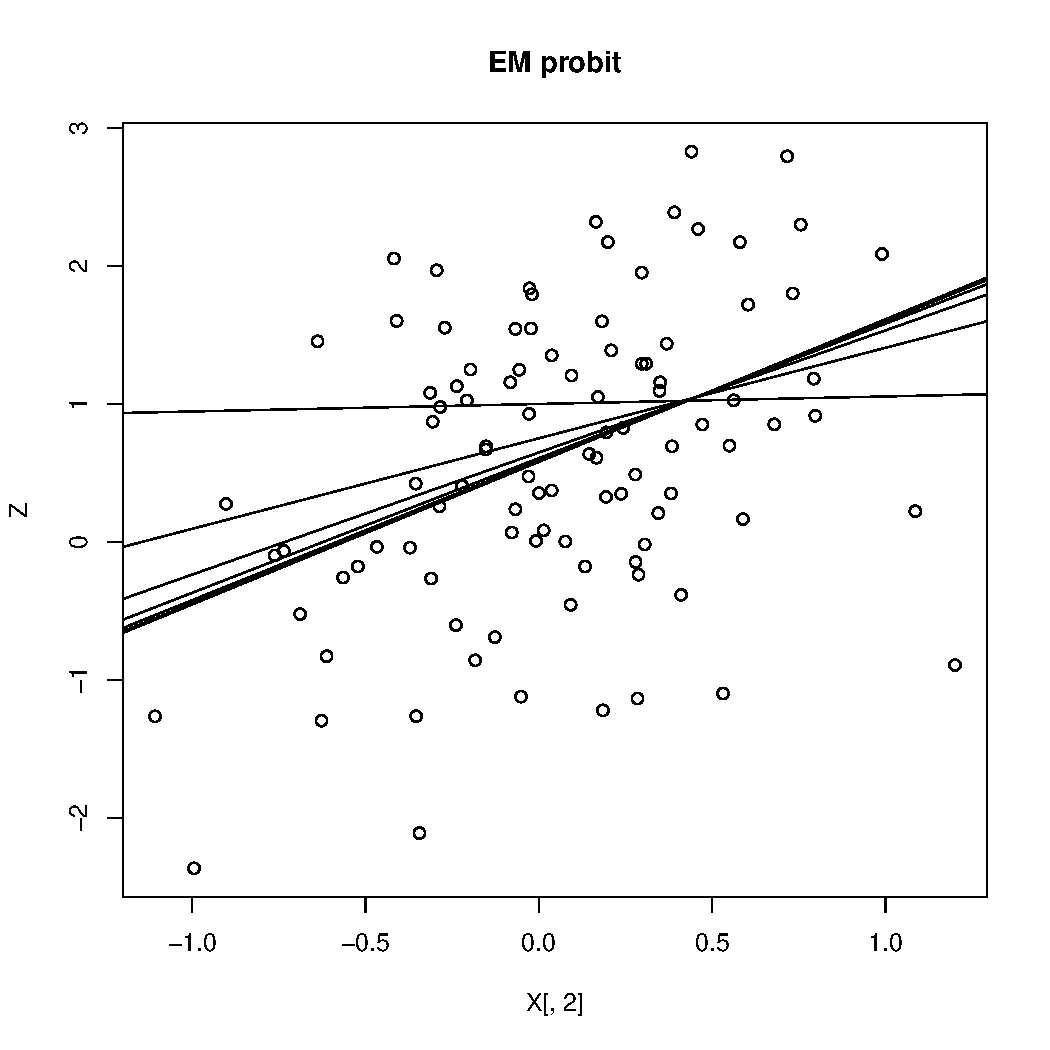
\includegraphics[width=\maxwidth]{figure/unnamed-chunk-13-1} 
\begin{kframe}\begin{verbatim}
## $beta
##                   [,1]
## (Intercept) 0.57934758
## X[, -1]1    1.03509061
## X[, -1]2    0.04487137
## X[, -1]3    0.01732625
## 
## $nit
## [1] 7
\end{verbatim}
\end{kframe}
\end{knitrout}
If $Z$ is observed, we can directly maximize the likelihood of the data, i.e. minimize the loss which is:
\begin{equation}
L(\beta)= (Z-X\beta)^T(Z-X\beta)
\end{equation}
In order to use the BGFS algorithm, we need the gradient of this loss function which is:
\begin{equation}
\frac{dL}{d\beta}(\beta)= -X^T Z+X^TX \beta
\end{equation}
The standard errors of the estimate $\hat{\beta}$ are given by the square root of the diagonal terms of the following matrix:
\begin{equation}
Est.Var[\hat{\beta}]=\frac{\hat{\epsilon}^T\hat{\epsilon}}{n-p}(X^TX)^{-1}
\end{equation}
\begin{knitrout}
\definecolor{shadecolor}{rgb}{0.969, 0.969, 0.969}\color{fgcolor}\begin{kframe}
\begin{alltt}
\hlcom{# data}
\hlstd{beta} \hlkwb{=} \hlkwd{matrix}\hlstd{(}\hlkwd{c}\hlstd{(}\hlnum{.5}\hlstd{,}\hlnum{1}\hlstd{,}\hlnum{0}\hlstd{,}\hlnum{0}\hlstd{),}\hlkwc{ncol}\hlstd{=}\hlnum{1}\hlstd{)}
\hlstd{X} \hlkwb{=} \hlkwd{cbind}\hlstd{(}\hlnum{1}\hlstd{,}\hlkwd{rnorm}\hlstd{(}\hlnum{100}\hlstd{,}\hlkwc{sd}\hlstd{=}\hlnum{.5}\hlstd{),}\hlkwd{rnorm}\hlstd{(}\hlnum{100}\hlstd{,}\hlkwc{sd}\hlstd{=}\hlnum{2}\hlstd{),}\hlkwd{rnorm}\hlstd{(}\hlnum{100}\hlstd{,}\hlkwc{sd}\hlstd{=}\hlnum{2}\hlstd{))}
\hlstd{Z} \hlkwb{=} \hlstd{X}\hlopt\hlstd{beta}\hlopt{+}\hlkwd{matrix}\hlstd{(}\hlkwd{rnorm}\hlstd{(}\hlnum{100}\hlstd{),}\hlkwc{ncol}\hlstd{=}\hlnum{1}\hlstd{)}
\hlstd{Y}\hlkwb{=}\hlstd{Z} \hlcom{# Observed data}

\hlcom{# BFGS}
\hlstd{loss} \hlkwb{=} \hlkwa{function}\hlstd{(}\hlkwc{beta}\hlstd{)\{}
  \hlstd{r}\hlkwb{=}\hlstd{Y}\hlopt{-}\hlstd{X}\hlopt\hlstd{beta}
  \hlkwd{sum}\hlstd{(r}\hlopt{^}\hlnum{2}\hlstd{)}\hlopt{/}\hlnum{2}
\hlstd{\}}
\hlstd{grad} \hlkwb{=} \hlkwa{function}\hlstd{(}\hlkwc{beta}\hlstd{)\{}
  \hlopt{-}\hlkwd{crossprod}\hlstd{(X,Y}\hlopt{-}\hlstd{X}\hlopt\hlstd{beta)}
\hlstd{\}}
\hlstd{beta0}\hlkwb{=}\hlkwd{apply}\hlstd{(X,}\hlnum{2}\hlstd{,mean)}
\hlstd{opt}\hlkwb{=}\hlkwd{optim}\hlstd{(}\hlkwc{par}\hlstd{=beta0,}\hlkwc{fn}\hlstd{=loss,}\hlkwc{gr}\hlstd{=grad,}\hlkwc{method}\hlstd{=}\hlstr{"BFGS"}\hlstd{)}
\hlstd{opt}
\end{alltt}
\begin{verbatim}
## $par
## [1]  0.51501717  1.15268959 -0.08365974  0.04815986
## 
## $value
## [1] 57.20076
## 
## $counts
## function gradient 
##       30        7 
## 
## $convergence
## [1] 0
## 
## $message
## NULL
\end{verbatim}
\begin{alltt}
\hlcom{# Standard errors}
\hlstd{beta_hat}\hlkwb{=}\hlstd{opt}\hlopt{$}\hlstd{par}
\hlkwd{sqrt}\hlstd{(}\hlkwd{diag}\hlstd{(}\hlkwd{sum}\hlstd{((Y}\hlopt{-}\hlstd{X}\hlopt\hlstd{beta_hat)}\hlopt{^}\hlnum{2}\hlstd{)}\hlopt{/}
            \hlstd{(}\hlnum{100}\hlopt{-}\hlnum{4}\hlstd{)}\hlopt{*}\hlkwd{solve}\hlstd{(}\hlkwd{crossprod}\hlstd{(X,X))))}
\end{alltt}
\begin{verbatim}
## [1] 0.11117243 0.18878526 0.05701767 0.05086372
\end{verbatim}
\end{kframe}
\end{knitrout}
There are less iterations for EM than for BGFS, 7 against approximately 30 here.


%%%%%%%%%%%%%%%%%%%%%%%%%%%%%%%%%%%%%
\section{Helical valley}
%%%%%%%%%%%%%%%%%%%%%%%%%%%%%%%%%%%%%
I define three slices, one in each direction and plot the corresponding 3d output:
\begin{knitrout}
\definecolor{shadecolor}{rgb}{0.969, 0.969, 0.969}\color{fgcolor}\begin{kframe}
\begin{alltt}
\hlcom{# Helical valley}
\hlstd{theta} \hlkwb{<-} \hlkwa{function}\hlstd{(}\hlkwc{x1}\hlstd{,}\hlkwc{x2}\hlstd{)} \hlkwd{atan2}\hlstd{(x2, x1)}\hlopt{/}\hlstd{(}\hlnum{2}\hlopt{*}\hlstd{pi)}

\hlstd{f} \hlkwb{<-} \hlkwa{function}\hlstd{(}\hlkwc{x}\hlstd{) \{}
  \hlstd{f1} \hlkwb{<-} \hlnum{10}\hlopt{*}\hlstd{(x[}\hlnum{3}\hlstd{]} \hlopt{-} \hlnum{10}\hlopt{*}\hlkwd{theta}\hlstd{(x[}\hlnum{1}\hlstd{],x[}\hlnum{2}\hlstd{]))}
  \hlstd{f2} \hlkwb{<-} \hlnum{10}\hlopt{*}\hlstd{(}\hlkwd{sqrt}\hlstd{(x[}\hlnum{1}\hlstd{]}\hlopt{^}\hlnum{2}\hlopt{+}\hlstd{x[}\hlnum{2}\hlstd{]}\hlopt{^}\hlnum{2}\hlstd{)}\hlopt{-}\hlnum{1}\hlstd{)}
  \hlstd{f3} \hlkwb{<-} \hlstd{x[}\hlnum{3}\hlstd{]}
  \hlkwd{return}\hlstd{(f1}\hlopt{^}\hlnum{2}\hlopt{+}\hlstd{f2}\hlopt{^}\hlnum{2}\hlopt{+}\hlstd{f3}\hlopt{^}\hlnum{2}\hlstd{)}
\hlstd{\}}

\hlstd{a}\hlkwb{=}\hlnum{0} \hlcom{#Define slice}
\hlstd{f1} \hlkwb{=} \hlkwa{function}\hlstd{(}\hlkwc{x2}\hlstd{,}\hlkwc{x3}\hlstd{)\{}
  \hlstd{m}\hlkwb{=}\hlkwd{cbind}\hlstd{(x2,x3)}
  \hlkwd{apply}\hlstd{(m,}\hlnum{1}\hlstd{,}\hlkwa{function}\hlstd{(}\hlkwc{row}\hlstd{)} \hlkwd{f}\hlstd{(}\hlkwd{c}\hlstd{(a,row)))}
\hlstd{\}}

\hlstd{b}\hlkwb{=}\hlnum{5} \hlcom{#Define slice}
\hlstd{f2} \hlkwb{=} \hlkwa{function}\hlstd{(}\hlkwc{x1}\hlstd{,}\hlkwc{x3}\hlstd{)\{}
  \hlstd{m}\hlkwb{=}\hlkwd{cbind}\hlstd{(x1,x3)}
  \hlkwd{apply}\hlstd{(m,}\hlnum{1}\hlstd{,}\hlkwa{function}\hlstd{(}\hlkwc{row}\hlstd{)} \hlkwd{f}\hlstd{(}\hlkwd{c}\hlstd{(row[}\hlnum{1}\hlstd{],b,row[}\hlnum{2}\hlstd{])))}
\hlstd{\}}

\hlstd{c}\hlkwb{=}\hlnum{5} \hlcom{#Define slice}
\hlstd{f3} \hlkwb{=} \hlkwa{function}\hlstd{(}\hlkwc{x1}\hlstd{,}\hlkwc{x2}\hlstd{)\{}
  \hlstd{m}\hlkwb{=}\hlkwd{cbind}\hlstd{(x1,x2)}
  \hlkwd{apply}\hlstd{(m,}\hlnum{1}\hlstd{,}\hlkwa{function}\hlstd{(}\hlkwc{row}\hlstd{)} \hlkwd{f}\hlstd{(}\hlkwd{c}\hlstd{(row,c)))}
\hlstd{\}}
\end{alltt}
\end{kframe}
\end{knitrout}
\begin{knitrout}
\definecolor{shadecolor}{rgb}{0.969, 0.969, 0.969}\color{fgcolor}\begin{kframe}
\begin{alltt}
\hlstd{x}\hlkwb{=}\hlkwd{seq}\hlstd{(}\hlopt{-}\hlnum{10}\hlstd{,}\hlnum{10}\hlstd{,}\hlkwc{by}\hlstd{=}\hlnum{0.5}\hlstd{)}
\hlkwd{persp}\hlstd{(x,x,}\hlkwd{outer}\hlstd{(x,x,f1),}\hlkwc{phi}\hlstd{=}\hlnum{20}\hlstd{,}\hlkwc{theta}\hlstd{=}\hlopt{-}\hlnum{15}\hlstd{)}
\end{alltt}
\end{kframe}
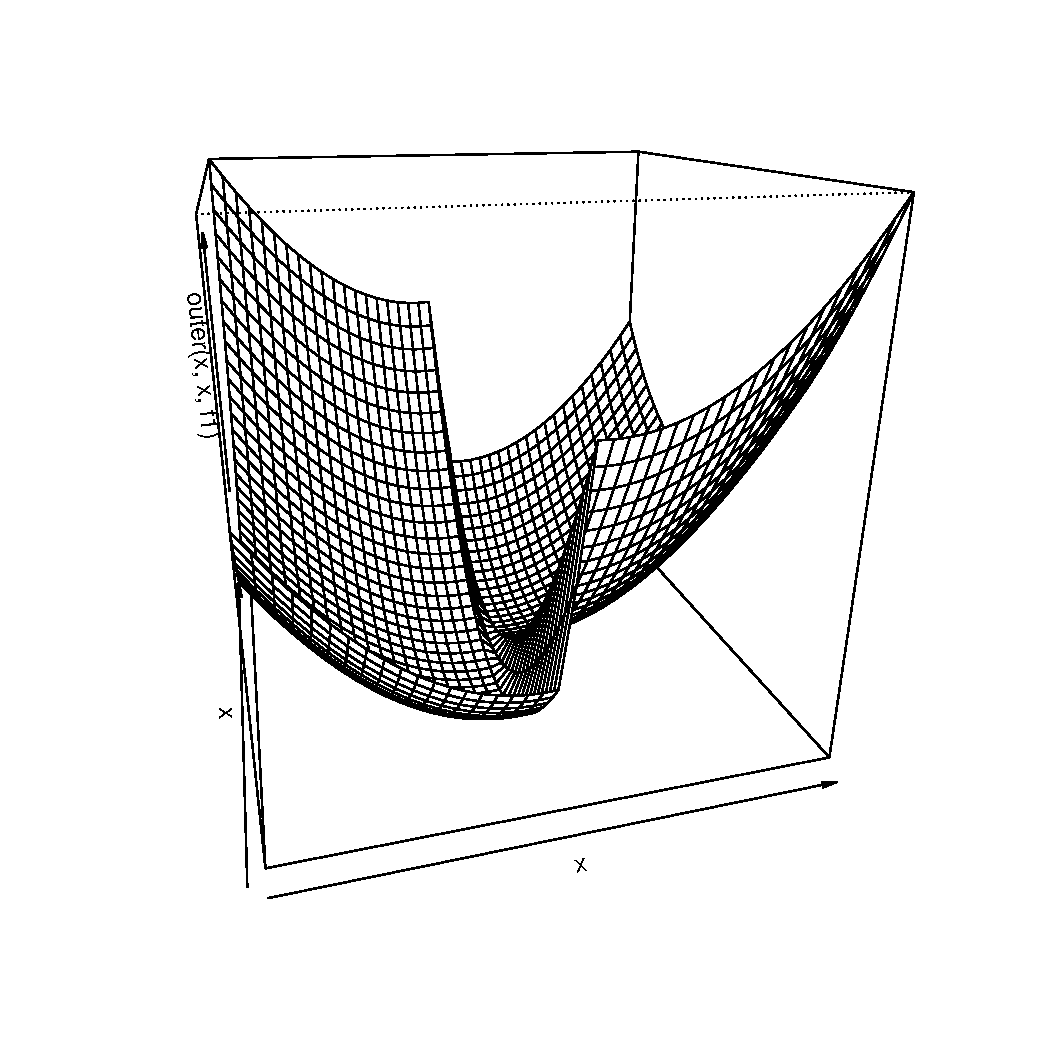
\includegraphics[width=\maxwidth]{figure/unnamed-chunk-16-1} 

\end{knitrout}
\begin{knitrout}
\definecolor{shadecolor}{rgb}{0.969, 0.969, 0.969}\color{fgcolor}\begin{kframe}
\begin{alltt}
\hlkwd{persp}\hlstd{(x,x,}\hlkwd{outer}\hlstd{(x,x,f2),}\hlkwc{phi}\hlstd{=}\hlnum{20}\hlstd{,}\hlkwc{theta}\hlstd{=}\hlopt{-}\hlnum{60}\hlstd{)}
\end{alltt}
\end{kframe}
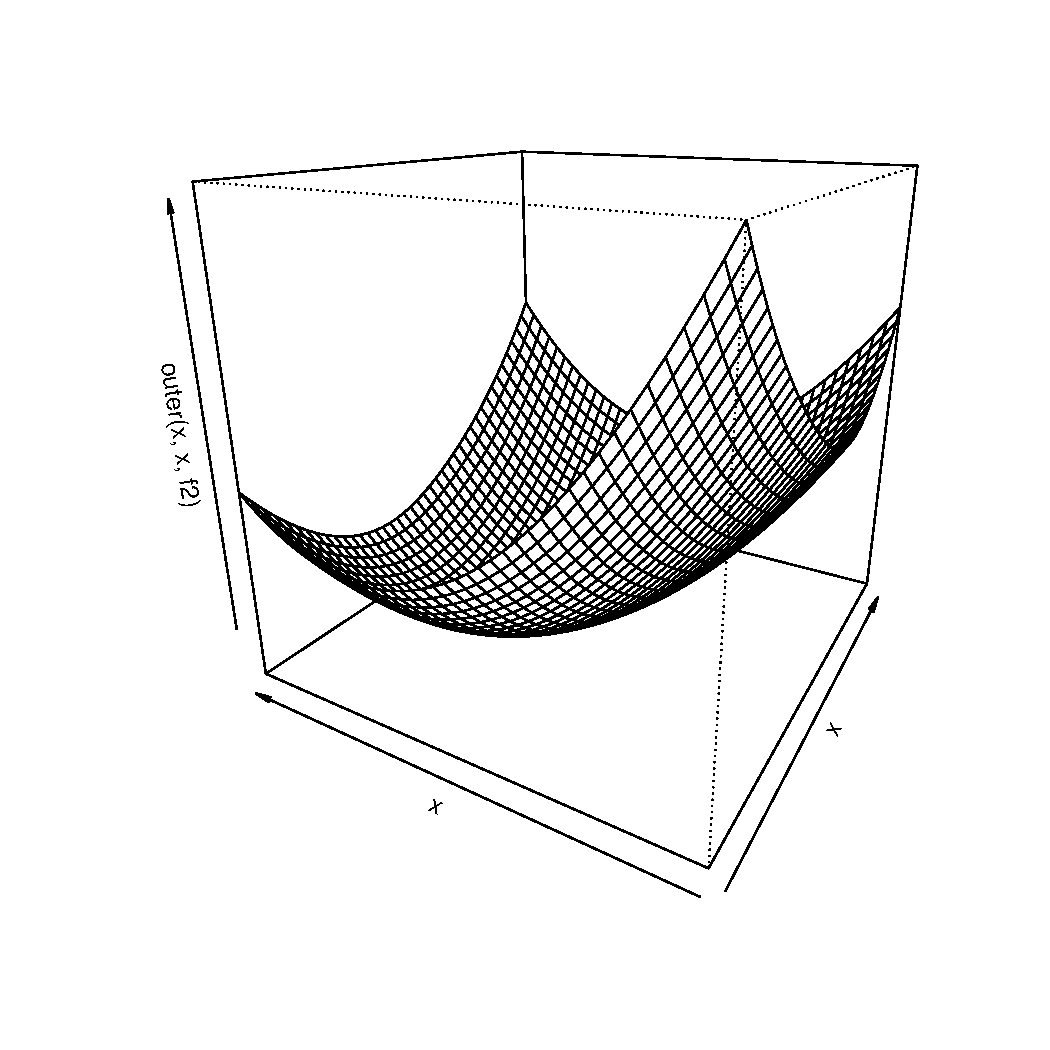
\includegraphics[width=\maxwidth]{figure/unnamed-chunk-17-1} 

\end{knitrout}
\begin{knitrout}
\definecolor{shadecolor}{rgb}{0.969, 0.969, 0.969}\color{fgcolor}\begin{kframe}
\begin{alltt}
\hlkwd{persp}\hlstd{(x,x,}\hlkwd{outer}\hlstd{(x,x,f3),}\hlkwc{phi}\hlstd{=}\hlnum{20}\hlstd{,}\hlkwc{theta}\hlstd{=}\hlopt{-}\hlnum{60}\hlstd{)}
\end{alltt}
\end{kframe}
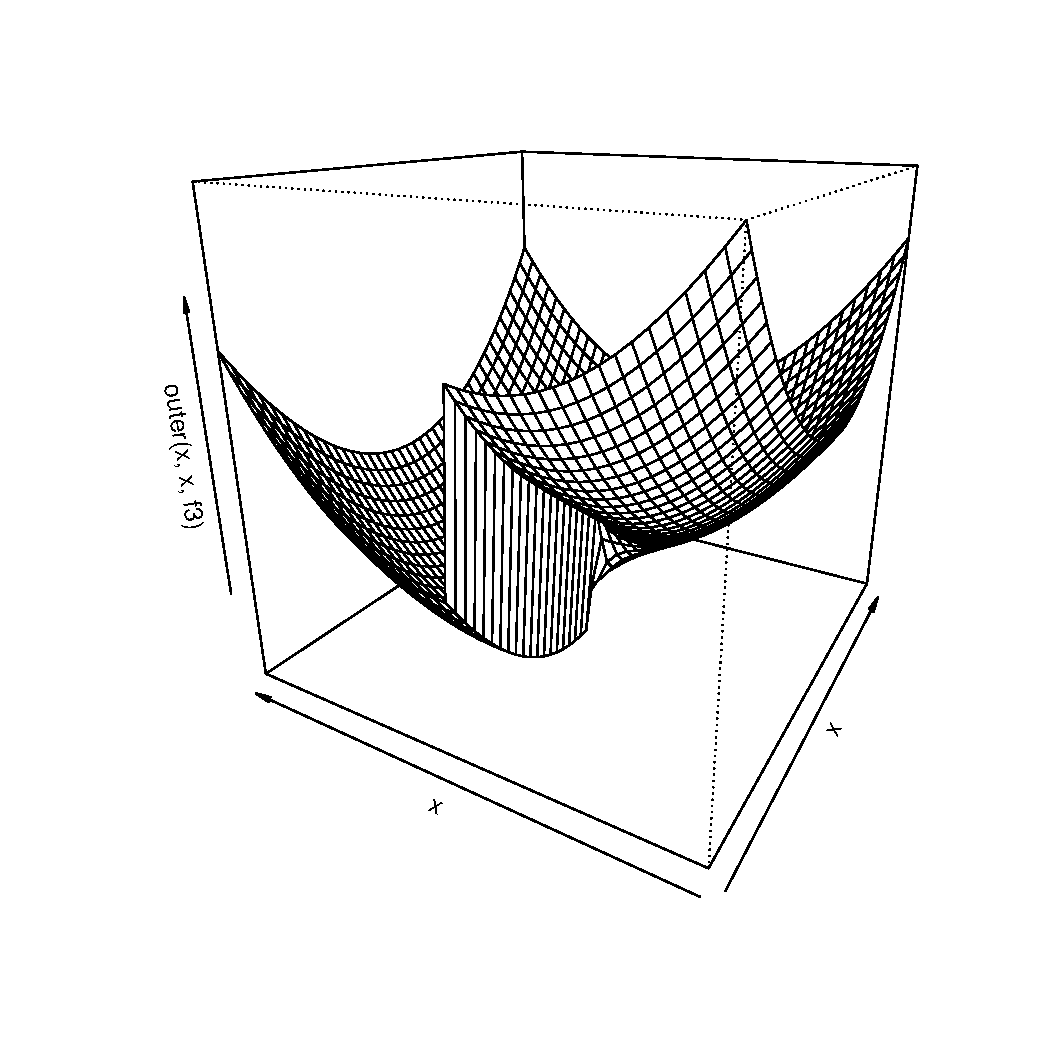
\includegraphics[width=\maxwidth]{figure/unnamed-chunk-18-1} 

\end{knitrout}
I can also plot a contourplot:
\begin{knitrout}
\definecolor{shadecolor}{rgb}{0.969, 0.969, 0.969}\color{fgcolor}\begin{kframe}
\begin{alltt}
\hlkwd{contour}\hlstd{(x,x,}\hlkwd{outer}\hlstd{(x,x,f1))}
\end{alltt}
\end{kframe}
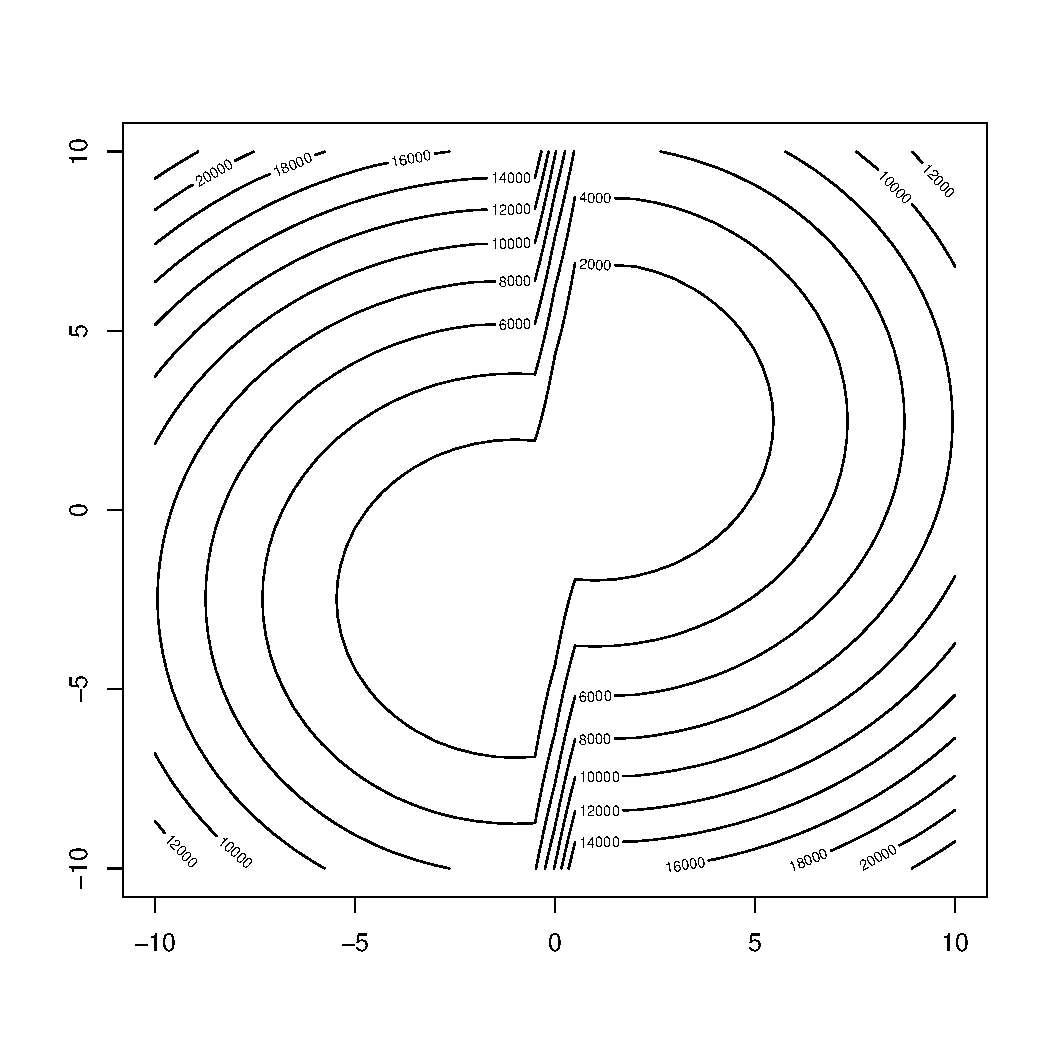
\includegraphics[width=\maxwidth]{figure/unnamed-chunk-19-1} 

\end{knitrout}
Finally, here are the results for two different initializations which lead to different outcomes. The first call may be more appropriate since the two methods (optim and lnm) lead approximately to the same result. However, for the second example it seems that another loal minima is reached.
\begin{knitrout}
\definecolor{shadecolor}{rgb}{0.969, 0.969, 0.969}\color{fgcolor}\begin{kframe}
\begin{alltt}
\hlcom{# Results}
\hlstd{x_init}\hlkwb{=}\hlkwd{c}\hlstd{(}\hlnum{1}\hlstd{,}\hlnum{1}\hlstd{,}\hlnum{1}\hlstd{)}
\hlkwd{optim}\hlstd{(x_init,f)}
\end{alltt}
\begin{verbatim}
## $par
## [1]  0.9999779414 -0.0001349269 -0.0001927127
## 
## $value
## [1] 1.343098e-07
## 
## $counts
## function gradient 
##      172       NA 
## 
## $convergence
## [1] 0
## 
## $message
## NULL
\end{verbatim}
\begin{alltt}
\hlkwd{max}\hlstd{(}\hlkwd{abs}\hlstd{(}\hlkwd{optim}\hlstd{(x_init,f)}\hlopt{$}\hlstd{par}\hlopt{-}\hlkwd{nlm}\hlstd{(f,x_init)}\hlopt{$}\hlstd{estimate))} \hlcom{#similar}
\end{alltt}
\begin{verbatim}
## [1] 6.258705e-05
\end{verbatim}
\begin{alltt}
\hlcom{# Different starting point}
\hlstd{x_init}\hlkwb{=}\hlkwd{c}\hlstd{(}\hlopt{-}\hlnum{20}\hlstd{,}\hlnum{100}\hlstd{,}\hlnum{1}\hlstd{)}
\hlkwd{optim}\hlstd{(x_init,f)}
\end{alltt}
\begin{verbatim}
## $par
## [1]  0.9618505 -0.2799601 -0.4494896
## 
## $value
## [1] 0.2025213
## 
## $counts
## function gradient 
##      101       NA 
## 
## $convergence
## [1] 0
## 
## $message
## NULL
\end{verbatim}
\begin{alltt}
\hlkwd{optim}\hlstd{(x_init,f)}\hlopt{$}\hlstd{par}\hlopt{-}\hlkwd{nlm}\hlstd{(f,x_init)}\hlopt{$}\hlstd{estimate} \hlcom{#different estimate}
\end{alltt}
\begin{verbatim}
## [1] -0.03814949 -0.27996007 -0.44948964
\end{verbatim}
\end{kframe}
\end{knitrout}










\end{document}















